\documentclass[conference]{IEEEtran}
\IEEEoverridecommandlockouts
% The preceding line is only needed to identify funding in the first footnote. If that is unneeded, please comment it out.
\usepackage{cite}
\usepackage{amsmath,amssymb,amsfonts}
\usepackage{algorithmic}
\usepackage{graphicx}
\usepackage{textcomp}
\usepackage{xcolor}
\def\BibTeX{{\rm B\kern-.05em{\sc i\kern-.025em b}\kern-.08em
    T\kern-.1667em\lower.7ex\hbox{E}\kern-.125emX}}
\begin{document}

\title{Knocking Down CAPTCHAs using Machine Learning models\\
{\footnotesize \textsuperscript}
}
\author{\IEEEauthorblockN{José Moreira}
\IEEEauthorblockA{\textit{Dep. de Eletrónica, Telecomunicações e Informática}\\
\textit{Universidade de Aveiro)}\\
Aveiro, Portugal \\
jcristianosm@ua.pt}
\and
\IEEEauthorblockN{Bruno Aguiar}
\IEEEauthorblockA{\textit{Dep. de Eletrónica, Telecomunicações e Informática} \\
\textit{Universidade de Aveiro}\\
Aveiro, Portugal \\ 
brunoaguiar@ua.pt}
}

\maketitle

\begin{abstract}
Completely Automated Public Turing test to tell Computers and Humans Apart (CAPTCHA) are  systems that allow to evaluate if a computing system is being controlled by a human or by a robot. CAPTCHAs are being used widely over the internet  to ensure the security of a system from being accessed by a bot over the network. In this paper, we will use machine learning models to crack down most of these CAPTCHAs as well as two different approaches to image processing and segmentation to feed these machine learning models.
\end{abstract}

\vspace{5mm}

\begin{IEEEkeywords}
Machine Learning, CNN, CAPTCHA, K-NN, Data Segmentation, Synthetic Data, Transfer Learning
\end{IEEEkeywords}

\section{Introduction}
\par CAPTCHAs are being widely used over the internet to protect websites against non/human entities. The most frequent CAPTCHA system used is text-based CAPTCHA, which is consisted by a random combination of upper and lower case letters from Aa to Zz and ten digits (0-9) with a big variety of transformations, distortions, where characters may be crowded together without spaces to make the \textit{digital life} of these ML agents more difficult. In addition, various geometric shapes are also added to introduce more noise and randomness to this system.
\par The algorithms used to create the CAPTCHA must be public[1], because it needs to demonstrate the robustness of the CAPTCHA and it needs to prove that it is a difficult problem for today's Artificial Intelligence (AI) models, rather just to discover the hidden algorithm obtained through reverse engineering.
\par Dechipering a CAPTCHA three fundamental things: 
\begin{itemize}
\item The capacity for consistent image recognition: Humans can identify the characters no matter what shape and size it appears
\item The capacity for image segmentation, which is the capacity to separate one character from another.
\item The capacity to parse images: Getting the context right to parse the CAPTCHA is fundamental.
\end{itemize}
\par The capability to detect CAPTCHA images is one of the most popular ways to benchmark AI systems, due to the hardness of the problem. If an AI system can crack a CAPTCHA, then it may also be capable of crack another complex AI problems. The purpose for these attacks can vary, but the most frequent ones are for account takeover (ATO), which is a method of credential theft for account takeover[2].

\section{State of the Art} 
During the research on the State of the Art for this particular subject, it is very clear that there are a pipeline to follow in other to crack down the CAPTCHA Problem, usually called \textit{The Decaptcha Pipeline}[3]. 
\param The first stage in this pipeline is the \textbf{Preprocessing}. In this stage, it is used several techniques to remote CAPTCHA's noise, confusing shapes and overall background. Most of this work is doing using Computer Vision techniques such as Morphological Transformations such as Erosion, Dilation, and Closing. The CAPTCHA is then binarized, and turned to black and white. \par The second stage is called the \textbf{Segmentation} stage and attempts to segment the CAPTCHAs with Color Filling Techniques, for example, as long as they are not contiguous. \par The next stage is the \textbf{Post-Segmentation}, and in this stage the letters are processed individually and its sized is normalized. Finally, the next final stages are the \textbf{Recognition}, to train the model classifier for every single character in the post-segmented dataset, and the \textbf{Post-Processing} stage, which is used to improve the model outcomes when its possible. Regardless the Recognition stage, the necessary and most used stages are the Preprocessing stage and the Post-Segmentation Stage, which enable to the model perform a single character prediction well enough. Although a technique that helps a lot and it's not widely used is the generation of new characters from the dataset to prevent over-fitting and increase the quality of the model. This technique is called \textbf{Data Augmentation} and there are two main methods to do it: Using \textbf{Oversampling}, in which it will replicate the minority classes to balance the dataset, and \textbf{SMOTE}, which is used to pseudo-random instances in the neighborhood of the minority classes.[3]
\par For the \textbf{recognition} problem, most of the classifiers today are more than enough, as they perform usually around 90-99.5\% for single characters. So, instead of searching for a classifier based only in performance, it is recommended to choose simple classifiers like the K Nearest Neighbors (KNN) and the State Vector Machine (SVM)[4]. Besides this recommendations, another famous classifiers for this problem is the use of Convolution Neural Networks (CNN), which give us slightly better results, but with the cost of being more computational intensive and more recently, and the use of Generative Adversarial networks (GAN), in which consists in two Neural networks competing in a zero-sum game with one being the agent's gain and the other being the agent's loss[5][6]. Although solvers can have an excellent performance on single character, CAPTCHAs are usually constituted by 5 letters and for being able to dodge this security mechanism, the model must be right in all of them, The changes to do so are lower in many cases, in a range of 30-96.5\% success rate (with +80\% being rare), which is still very alarming to the security of these CAPTCHAs."

\section{Dataset and Data Processing} 
Our dataset is composed by 1070 samples of CAPTCHA Images and with an alphabet of 19 characters. To pre-process these images we choose two ways of doing it. The classical approach of applying Computer Vision techniques to remove the noise and background shapes, and other approach followed by the book \textit{Hands On Machine Learning for CyberSecurity}. For the first approach we started by transforming the image to a gray scale and then turned it to a black and white image. A chain of Morphological Transformations were applied such as \textbf{Adaptive Thresholding}, \textbf{Closing} (Dilation followed by Erosion) and \textbf{Blurring}. After that we manually cropped the image into five sub-images, meaning the five letters present in the CAPTCHA (Figure 2).
\par In the second approach, we did not used any Morphological Transformations rather than converting the images to black and white and perform an automatic cropping to each single character. Because of this, the dataset was drastically reduced to ~300 samples. To overcome this situation, we implemented Transfer Learning, as we are going to talk more  about later on. 

\begin{center}
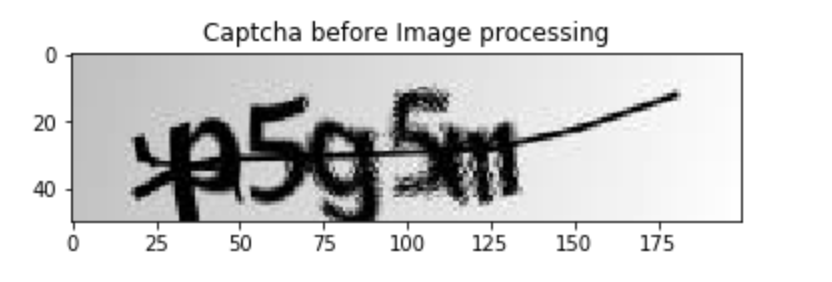
\includegraphics[scale=0.55]{Screenshot 2021-06-30 at 21.20.40.png}
\caption{Figure 1: Captcha before Image Processing}
\end{center}
\\ \\ \\
\begin{center}
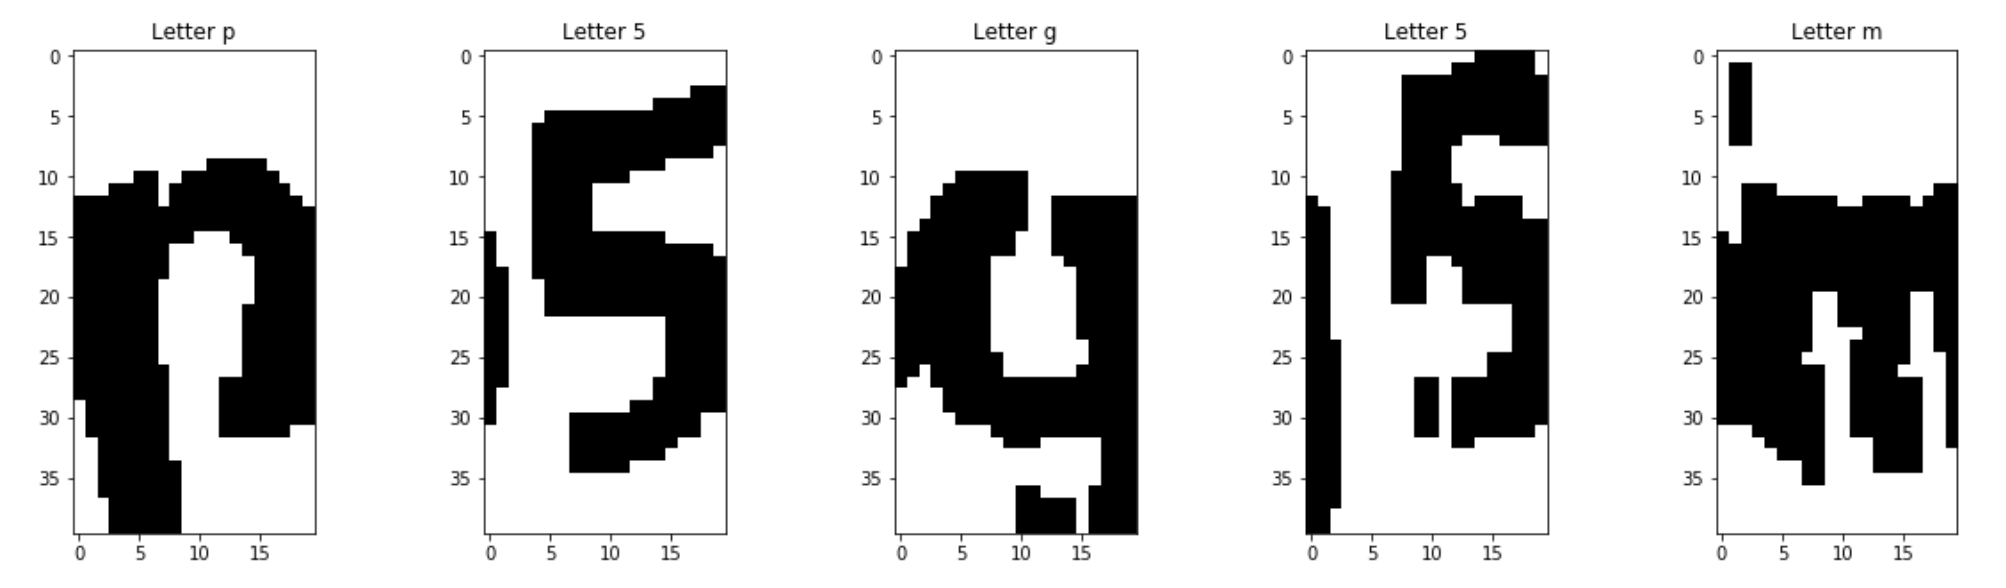
\includegraphics[scale=0.20]{Screenshot 2021-06-30 at 21.29.42.png}

\caption{Figure 2: Captcha after Image Processing}
\end{center}
\par

\section{Data Augmentation and Oversampling}
Data Augmentation is any technique that allow us to increase the amount of data images by creating modified synthetic ones from existing data. It helps us to prevent over-fitting. In this project we implemented a SMOTE technique that is going to generate synthetic samples from the minority class. With the augmented dataset, we decided to generate a few more samples, by changing the angle of the existing ones through \texttt{ImageDataGenerator}. 

\section{One Hot Encoding}
As a multi classification problem, we have an alphanumeric combination of 19 characters. There is a need for our input/output values to be numeric, so it was implemented the One-Hot Encoding to encode the categorical output labels.

\section{Data Splitting into Train, Validation and Test Sets}

To prevent any overfitting, and accomplish the best results, the data was divided in 2 new sets (80/20 split), a training set, used to train our models and a testing set to evaluate possible over or under fittings. We also perform a validation test splitting (50/50 split) when creating the test set and it's used in the CNN model.

\section{CNN}

Our CNN model is formed by 4 Conv layers and 3 FC layers with softmax output, with 1,013,683 of total parameters. In the Conv layers, we used a 3x3 kernel filter, padding with the value \texttt{same} such that output has the same height/width dimension as the input, activation function being ReLU, normalization of the results and performing Max Pooling to speed up the computation results. 
\par In the Fully Connected layers, we also used the ReLU activation function with normalization of the results and we also added a Dropout layer of 0.5 to prevent over-fitting.
\par For the loss function we went to  \texttt{categorical\_crossentropy} and for the optimizer of the input weights we went to \texttt{Adam} which seemed the best for this case.  
\par To ensure that our model keeps the learning rate in pace, we used the callback \texttt{ReduceLROnPlateau} to reduce the learning rate when our model stops improving.
\par Running the current model configuration, we were able to get an weighted average of 88\% on the character prediction and 87\% in the weighted F1-Score, with some characters reaching 100\% of accuracy like \textbf{y} and \textbf{3}, which is pretty impressive and in touch of the modern classifiers.
\begin{center}
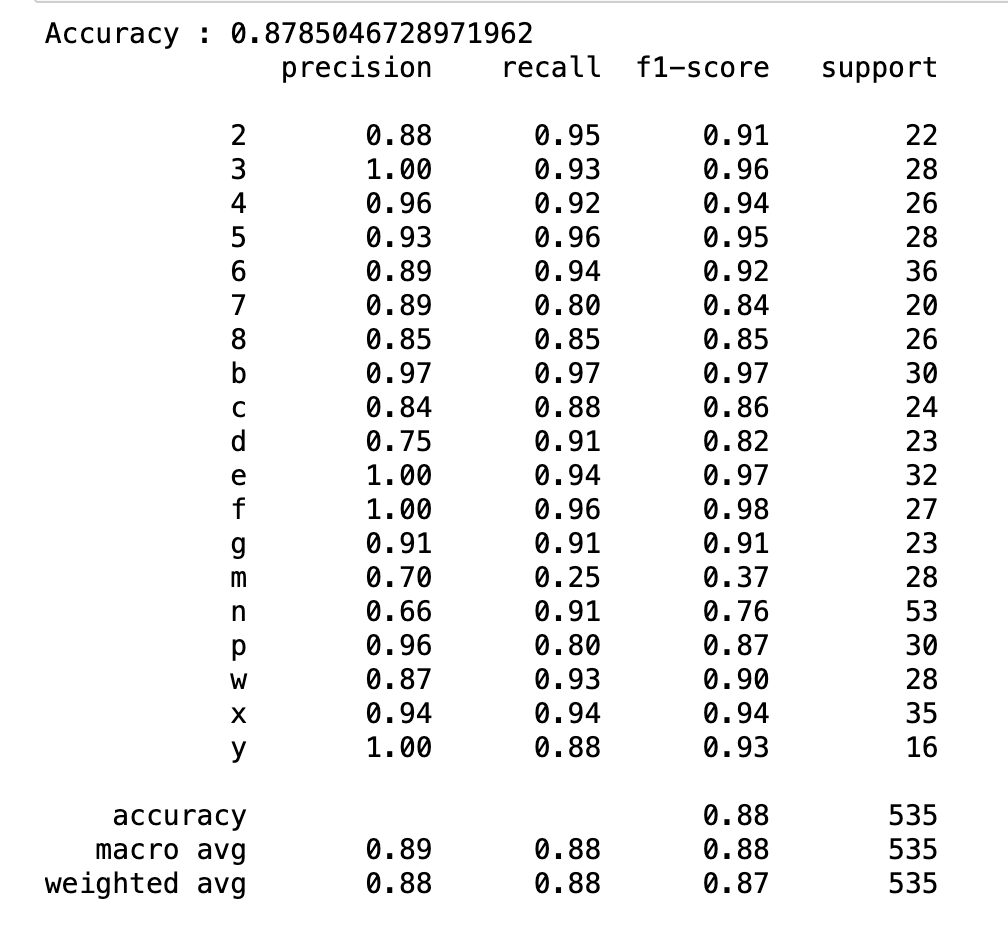
\includegraphics[scale=0.55]{cnn.png}
\caption{Figure 3: Accuracy and the report of CNN.}
\end{center}
\\ \\ \\


\section{KNN}
The K-Nearest Neighbors is a model used for both classification and regression. To use the K-Nearest Neighbors we had to reshape our training and testing data, as the model was not compatible with what we previous had. To accomplish this, we turned our arrays into two dimensional arrays, with number of elements in one, multiplication of the dimensions of each image in the other.  
With usable data, we iterated from 1 to 20, with the number iterating being the k value, to find the value that had the better results. After this iteration, we had this graph to display:
\begin{center}
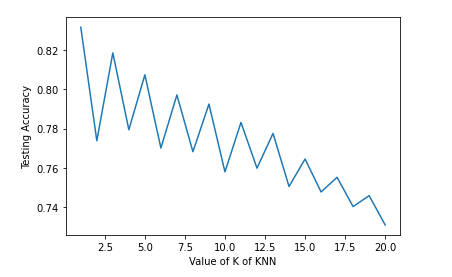
\includegraphics[scale=0.55]{knn.png}
\caption{Figure 4: Accuracy and value of K relation.}
\end{center}
\\ \\ \\
It was possible to notice that the higher the value, less the accuracy, therefore, the best value for the model would be 1. We ran the model again, with 1 as the k value, to present its accuracy and report. \begin{center}
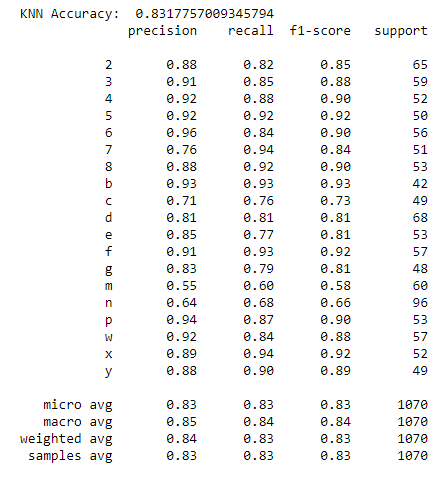
\includegraphics[scale=0.55]{knnreport.png}
\caption{Figure 5: Accuracy and report of KNN.}
\end{center}
\\ \\ \\
We obtained an 83\% accuracy with this model, that, even though is not that bad, it is clearly inferior to the values obtained in the CNN model. This results will be further analyzed ahead, when we actually solve CAPTCHAs using these models. 

\section{K-Fold Validation}
For the K-Fold Validation, we used 5 splits, with shuffle. After obtaining our arrays, for both testing and training, and for both x and y, we ran into a similar issue and in KNN. The format of the arrays were not compatible. Therefore, the same solution was applied, a reshape in the arrays, where they would become a two dimensional array, with the number of elements in one, and the multiplication of the dimensions of the image in the other. Using the KNN model developed previously, we were able to calculate what we needed for our Confusion Matrices. As said previously in this report, our dataset has 19 alphanumerical digits, therefore, our confusion matrices even though is two dimensional, is divided 19x19, describing the results provided by the kNN model. These are the matrices in question: 
\begin{center}
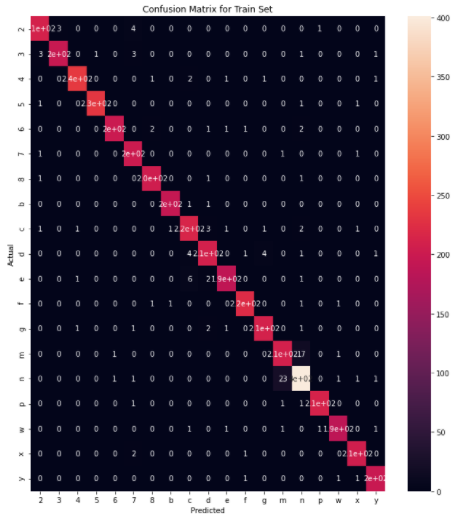
\includegraphics[scale=0.55]{confusionmatrix.png}
\caption{Figure 6: Confusion Matrix Train Set.}
\end{center}
\\ \\ \\
\begin{center}
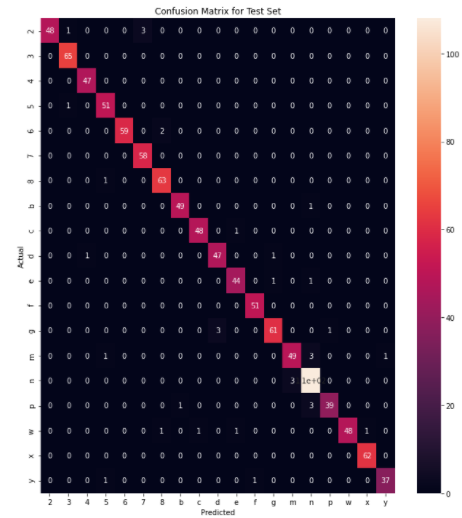
\includegraphics[scale=0.55]{confusionmatrix2.png}
\caption{Figure 7: Confusion Matrix Test Set.}
\end{center}
\\ \\ \\
The results are quite satisfactory, since there is a clear diagonal line, meaning the predicted value was the actual value most of the times, in every example. When the prediction was not spot on, there was only two or three cases where the model mistook a letter and or number more than 2 times, without the cases that we will talk about right now. . There are some huge exceptions on this success, in letters that have some similarities, namely 'm' and 'n' and 'c' and 'd'. This is, however, expected, because of said similarities.

\section{Testing and Resolving CAPTCHAs}
To test our models, we developed some specific methods to try and resolv the CAPTCHAs. The process was very simple, in each method (one for CNN and other for KNN) we provided the path to an image, the method, through cv2 would read the image, divide said image into fize different zones, where the letters usually are and add that information to an array. This array would after be used to predict the text in the CAPTCHA. To be easier to visualize, here is and example of a CAPTCHA being solved by both CNN and KNN models.  
\begin{center}
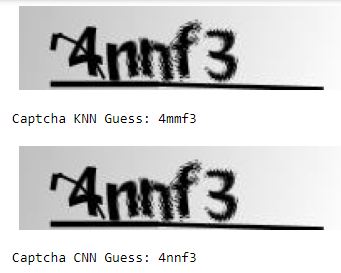
\includegraphics[scale=0.55]{captchasolved.png} \\
\caption{Figure 8: CAPTCHA Guess.}
\end{center}
\\ \\ \\
This example was used on purpose. Here, we can see two things. CNN is, in fact, more reliable, as it could crack a CAPTCHA KNN could not, and that the letters 'n' and 'm' are actually harder to predict. This however was not enough to test our models, therefore other methods were applied. This time, the purpose was different, we could already tell the CNN model provided better results, so we wanted to test and calculate the percentage of CAPTCHAs and letters it could predict. To do this, we had two approaches, one where we would slightly process the image, and other where we would just read the image and predict. To do this, we iterated through our entire dataset, of 1070 CAPTCHAs, and with each CAPTCHA being formed by 5 letters, 5350 letters to identify. Starting from the raw images, the results are slightly disappointing, because the model could only guess 4468 letters out of the 5350 possible, giving a 83.\% accuracy, number that quickly drops when we see the CAPTCHAs results, where it could only guess 521 out of 1070, meaning it had 48.6\% accuracy. However, these numbers are considerably higher when some sort of image processing is made. With the same dataset, the same iterations, the same letters and CAPTCHAs, with a little of image processing before the prediction,the model could get 4925 out of the 5030 letters right, meaning it had 92.0\% accuracy in letter identification and could solve 811 out of 1070 CAPTCHAs, meaning a 75.8\% solving accuracy. The solving accuracy may seem low, but we considered that only one fail out of 5 would be enough to fail, since that is what would happen in a real case. Many of the failed cases were actually very close to be solved, with 4 letters guessed correctly out of the 5. To facilitate the results visualization:
\begin{center}
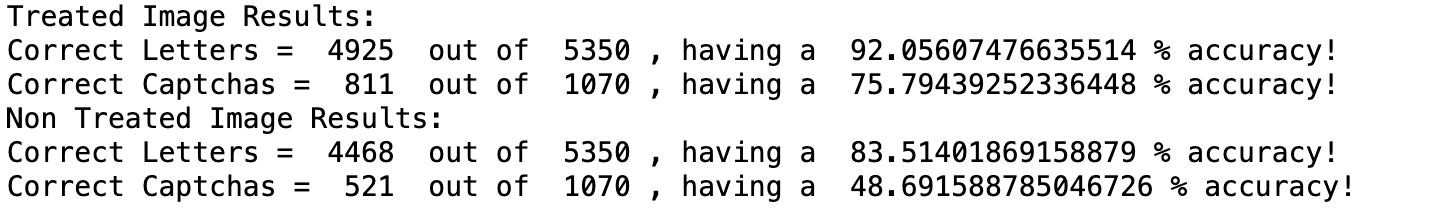
\includegraphics[scale=0.375]{newresults.png} 
\caption{Figure 9: Guessing Results.}
\end{center}
\\ \\ \\

\section{Second Approach for Data Processing and Transfer Learning}
As we said earlier in the paper, we followed a technique of Data processing in the book \textit{"Hands On Machine Learning for CyberSecurity”}, in which did not have many data processing techniques rather than transforming the image to black and White, find the contours of the CAPTCHA and, based on the ratio between the width and the height, crop the image into several letters. Because of that ratio, many images where dropped out, and remained only 484 samples, which is little in comparison with the previous data processing. We have tested with the dataset a CNN model, but the results showed poorly. To overcome this situation, and to learn more about, we applied Transfer Learning with the dataset to see if it performs well, but the performance did not improved (the accuracy was around 4-7\%). Although, we see this field with potential, saving a lot of time, effort, and possibly one of the keys to achieve the so desired AGI (Artificial General Intelligence).

\section{Conclusion}
Regarding work distribution, Bruno Aguiar has done Transfer Learning, Image Processing, CNN, José Moreira has done KNN, Image Processing and Testing, and everything else was done by both students simultaneously. Considering the results obtained, it is fair to say the CNN model is much better than the KNN in this particular case, and that should be the one to use in this kind of problems. Regarding the final results themselves, we are fairly pleased with the outcome. Considering the size of the dataset (not just in size, also in variety, since we only identified 19 alphanumerical characters instead of the expected 36, even though this was not the reason that dropped the accuracy since said letters were not there to be guessed as well) 92.0\% is actually a very good result. As said before the 75.8\% accuracy in solving the whole CAPTCHA may seem underwhelming but considering that just 1 failed guess out of of the 5 letters each one has was enough to fail at that CAPTCHA, it actually is not that bad. Comparing to what was said in the State of The Art, CAPTCHA solvers these days have around 30-96.5\% success rate, therefore our results were way above the average. 

\section{Notes}
To run the project, it is necessary to have the Jupyter Notebook file, the directory \texttt{samples} and the trained model \texttt{result\_model.h5} in the same directory. The model training process (\texttt{model.fit}) is commented in the Notebook file, because it takes too long to run, so it's key to have all files in the same directory, and everything can be imported as it should. 
\begin{thebibliography}{00}
\bibitem[1]{b1} "CAPTCHA" (May 2021). Wikipedia 
\bibitem[2]{b2} "Hands On Machine Learning for CyberSecurity" (December 2018)
\bibitem[3]{b3} Vasileios Iosifidis and Eirini Ntoutsi "Dealing with Bias via Data Augmentation in Supervised Learning Scenarios"
\bibitem[4]{b4} Elie Bursztein, Matthieu Martin, and John C. Mitchel "Text-based CAPTCHA Strengths and Weaknesses"
\bibitem[5]{b5} Ye, G, Tang, Z, Fang, D et al. (6 more authors) (2020) "Using Generative Adversarial Networks to Break andProtect Text Captcha"
\bibitem[6]{b6} Guixin Ye, Yansong Feng, D et al. (4 more authors) "Yet Another Text Captcha Solver:A Generative Adversarial Network Based Approach"
\end{thebibliography}

\end{document}
